\documentclass{article}
\usepackage{tikz}
\usetikzlibrary{arrows.meta}
\usetikzlibrary{intersections}


\begin{document}
    \begin{center}
        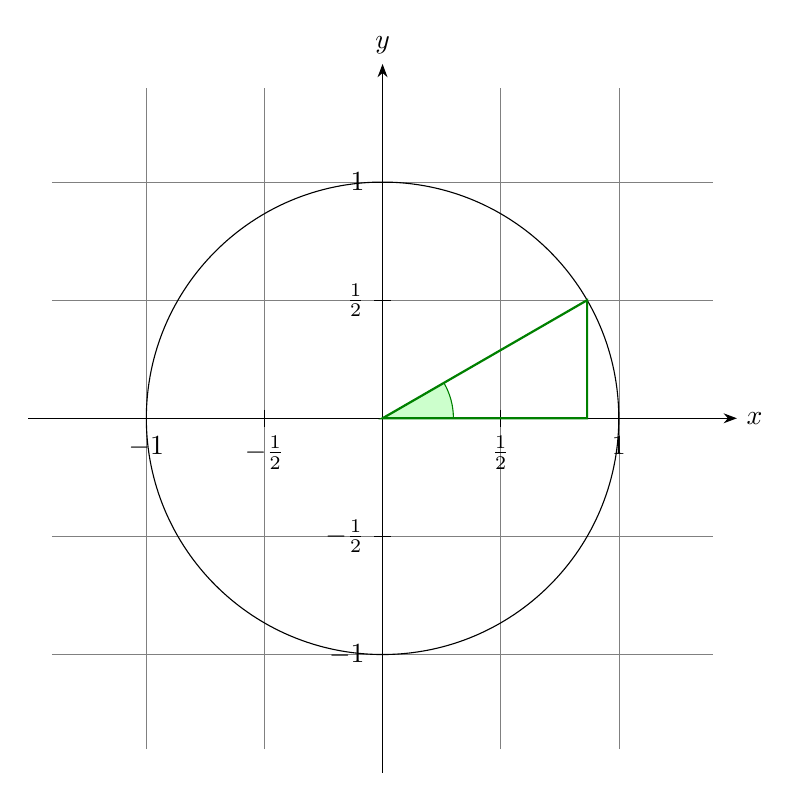
\begin{tikzpicture}[scale=3, >=Stealth]
            \draw[step=.5cm, help lines] (-1.4, -1.4) grid (1.4, 1.4);
            \draw[->] (-1.5, 0) -- (1.5, 0) node[anchor=west]{$x$};
            \draw[->] (0, -1.5) -- (0, 1.5) node[anchor=south]{$y$};
            \draw (0, 0) circle[radius=1cm];

            \foreach \x/\xtext in {-1, -0.5/-\frac{1}{2}, 0.5/\frac{1}{2}, 1}
                \draw (\x cm, 1pt) -- (\x cm, -1pt) node[anchor=north]{$\xtext$};
            \foreach \y/\ytext in {-1, -0.5/-\frac{1}{2}, 0.5/\frac{1}{2}, 1}
                \draw (1pt, \y cm) -- (-1pt, \y cm) node[anchor=east]{$\ytext$};

            \filldraw[fill=green!20!white, draw=green!50!black] (0, 0) -- (3mm, 0) arc[start angle=0, end angle=30, radius=3mm] -- cycle;

            \draw[green!50!black, thick] (0, 0) -- (30:1cm) -- (30:1cm|-0,0) -- cycle;
        \end{tikzpicture}
    \end{center}
\end{document}